% BÁO CÁO GIỮA KỲ: toàn bộ slide nằm trong file này. Biên dịch 2 lần: xelatex slide_giuaky.tex
% Bố cục và tông màu UIT theo chuẩn temp_uit_slide.md; có fallback nếu thiếu fonts/ hoặc assets/.
\documentclass[aspectratio=169,9pt]{beamer}
\usepackage{fontspec}
\usepackage[vietnamese]{babel}
\usepackage{amsmath,amssymb}
\usepackage{tikz}
\usetikzlibrary{calc,arrows.meta,positioning,fadings}
\usepackage[most]{tcolorbox}
\usepackage{booktabs,tabularx,colortbl,array,graphicx}
\newcolumntype{Y}{>{\raggedright\arraybackslash}X}

% ── Fonts: Be Vietnam Pro (không dùng Bungee), có fallback khi thiếu thư mục fonts/ ──
\IfFileExists{fonts/BeVietnamPro-Regular.ttf}{%
  \setsansfont{BeVietnamPro-Regular.ttf}[Path=fonts/, Ligatures=TeX,
    BoldFont=BeVietnamPro-Bold.ttf, ItalicFont=BeVietnamPro-Medium.ttf,
    BoldItalicFont=BeVietnamPro-SemiBold.ttf]
  \setmainfont{BeVietnamPro-Regular.ttf}[Path=fonts/, Ligatures=TeX,
    BoldFont=BeVietnamPro-Bold.ttf, ItalicFont=BeVietnamPro-Medium.ttf,
    BoldItalicFont=BeVietnamPro-SemiBold.ttf]
  \newfontfamily\hdsemi{BeVietnamPro-SemiBold.ttf}[Path=fonts/, Ligatures=TeX]
  \newfontfamily\hdheavy{BeVietnamPro-Bold.ttf}[Path=fonts/, Ligatures=TeX, FakeBold=1.6]
}{%
  \newcommand{\hdsemi}{\bfseries}
  \newcommand{\hdheavy}{\bfseries}
}
\newcommand{\bungee}{\hdheavy}
\newcommand{\bevnsemi}{\hdsemi}
\usefonttheme{professionalfonts}

% ── Bảng màu UIT (theo temp_uit_slide.md + tên màu tương thích sơ đồ cũ) ──
\definecolor{hdnavy}{HTML}{1B2C8C}
\definecolor{hdblue}{HTML}{0A6FBA}
\definecolor{hddeep}{HTML}{14276B}
\definecolor{hdink}{HTML}{14276B}
\definecolor{hdsky}{HTML}{D4E6FB}
\definecolor{hdpale}{HTML}{EAF2FD}
\definecolor{hdyellow}{HTML}{FFC21E}
\definecolor{hdlemon}{HTML}{FFE37A}
\definecolor{hdgold}{HTML}{FFC21E}
\definecolor{hdbrown}{HTML}{7A2E0E}
\definecolor{hdred}{HTML}{B31217}
\definecolor{hdgray}{HTML}{66728F}

\colorlet{inkblue}{hdnavy}
\colorlet{brandblue}{hdblue}
\definecolor{midblue}{HTML}{2E7DD1}
\definecolor{skyblue}{HTML}{73A5E1}
\colorlet{paleblue}{hdsky}
\colorlet{bgblue}{hdpale}
\colorlet{gold}{hdyellow}
\colorlet{footernavy}{hddeep}
\colorlet{textred}{hdred}
\definecolor{okgreen}{RGB}{0,120,60}

% Logo chỉ chèn khi file tồn tại
\newcommand{\logoimg}[1]{\IfFileExists{assets/hoids1_logo.png}{\includegraphics[height=#1]{assets/hoids1_logo.png}}{}}

% Chèn ảnh có khung giữ chỗ
\newcommand{\slideimg}[3][0.9\textwidth]{%
  \IfFileExists{images/#2}{%
    \includegraphics[width=#1,height=0.48\textheight,keepaspectratio]{images/#2}%
  }{%
    \fcolorbox{skyblue}{white}{\parbox[c][0.26\textheight][c]{#1}{\centering\scriptsize\color{inkblue}%
      \textbf{[CHƯA CÓ ẢNH]}\\[2pt]\texttt{images/#2}\\[2pt]#3}}%
  }%
}

\usetheme{default}
\setbeamertemplate{navigation symbols}{}
\setbeamercolor{normal text}{fg=hdink}
\setbeamercolor{structure}{fg=hdblue}
\setbeamercolor{itemize item}{fg=hdblue}
\setbeamercolor{itemize subitem}{fg=hdgold}
\setbeamertemplate{itemize item}{\color{hdblue}\small\textbullet}
\setbeamertemplate{itemize subitem}{\color{hdgold}\scriptsize\textbullet}
\setbeamersize{text margin left=3.2mm, text margin right=3.2mm}
\setlength{\parindent}{0pt}
\renewcommand{\baselinestretch}{1.02}

\setbeamercolor{block title}{bg=hdnavy,fg=hdlemon}
\setbeamercolor{block body}{bg=white,fg=hdink}
\setbeamercolor{block title alerted}{bg=hdblue,fg=white}
\setbeamercolor{block body alerted}{bg=white,fg=hdink}
\setbeamercolor{block title example}{bg=hdyellow,fg=hdbrown}
\setbeamercolor{block body example}{bg=white,fg=hdink}
\setbeamerfont{block title}{family=\hdsemi,size=\footnotesize}
\setbeamerfont{block title example}{family=\hdsemi,size=\footnotesize}
\setbeamerfont{block title alerted}{family=\hdsemi,size=\footnotesize}
\setbeamertemplate{blocks}[rounded][shadow=false]

% ── Thẻ nội dung tcolorbox (theo temp_uit_slide.md) ──
\tcbset{hdbase/.style={enhanced, colback=white, boxrule=0.8pt, arc=2mm, left=2mm, right=2mm, top=2.4mm, bottom=1mm,
  before skip=2mm, after skip=0.4mm, fontupper=\scriptsize, coltext=hdink, fonttitle=\bfseries\scriptsize,
  attach boxed title to top left={xshift=2mm, yshift*=-\tcboxedtitleheight/2},
  boxed title style={arc=1.4mm, boxrule=0pt, left=1.6mm, right=1.6mm, top=0.35mm, bottom=0.35mm},
  before upper={\setlength{\parskip}{1.4pt}}}}
\newtcolorbox{khung}[2][]{hdbase, colframe=hdyellow, colbacktitle=hdnavy, coltitle=hdlemon, title={#2}, #1}
\newtcolorbox{luuy}[2][]{hdbase, colframe=hdred!75, colbacktitle=hdred, coltitle=white, title={#2}, #1}
\newtcolorbox{ketluan}[1][]{enhanced, colframe=white, boxrule=0.8pt, arc=2.4mm, interior style={top color=hdlemon, bottom color=hdgold},
  coltext=hdbrown, fontupper=\bfseries\scriptsize, halign=flush center, left=2mm, right=2mm, top=0.6mm, bottom=0.6mm, before skip=1.4mm, after skip=0.4mm, #1}

\newenvironment{haicot}[1]{\begin{columns}[T,onlytextwidth]\begin{column}{#1\textwidth}}{\end{column}\end{columns}}
\newcommand{\sang}[1]{\end{column}\begin{column}{#1\textwidth}}
\newcommand{\bs}[1]{\tikz[baseline=(hdbs.base)]\node[circle,fill=hdblue,inner sep=1pt,minimum size=3.4mm,font=\bfseries\fontsize{6.4}{7}\selectfont,text=hdlemon](hdbs){#1};\ }
\newcommand{\sao}[3]{\fill[hdyellow] (#1,#2) ++(0,#3) .. controls +(0.02*#3,-0.6*#3) and +(-0.6*#3,0.02*#3) .. ++(#3,-#3) .. controls +(-0.6*#3,-0.02*#3) and +(0.02*#3,0.6*#3) .. ++(-#3,-#3) .. controls +(-0.02*#3,0.6*#3) and +(0.6*#3,-0.02*#3) .. ++(-#3,#3) .. controls +(0.6*#3,0.02*#3) and +(-0.02*#3,-0.6*#3) .. ++(#3,#3) -- cycle;}

% ── Nền: chuyển sắc xanh nhạt + cột mờ sát đáy ──
\setbeamertemplate{background}{%
  \begin{tikzpicture}
    \useasboundingbox (0,0) rectangle (\paperwidth,\paperheight);
    \shade[top color=hdpale, bottom color=hdsky] (0,0) rectangle (\paperwidth,\paperheight);
    \foreach \x/\h in {0.1/0.85,1.0/0.55,1.9/0.7,10.9/0.5,11.8/0.75,12.7/0.55,13.6/0.9,14.5/0.65,15.3/1.0}{
      \fill[hdblue,opacity=0.07,rounded corners=1pt] (\x,0.34) rectangle ++(0.7,\h);}
  \end{tikzpicture}%
}

% ── Tiêu đề trang: MỘT DÒNG, cao 0,84 cm ──
\newcommand{\machuyende}{NT106}
\setbeamertemplate{frametitle}{%
  \nointerlineskip
  \hspace*{-3.2mm}\begin{tikzpicture}
    \useasboundingbox (0,0) rectangle (\paperwidth,0.84);
    \fill[white,opacity=0.78] (0,0.04) rectangle (\paperwidth,0.84);
    \node[anchor=west,rounded corners=2.6pt,left color=hdblue,right color=hdnavy,text=hdlemon,inner xsep=5pt,inner ysep=2.6pt,font=\bfseries\footnotesize] (ma) at (0.3,0.45) {\machuyende};
    \node[anchor=west,text=hdnavy,font=\hdheavy\fontsize{11}{12}\selectfont] at ($(ma.east)+(0.14,0)$) {\insertframetitle};
    \node[anchor=east,text=hdgray,font=\hdsemi\fontsize{6.8}{8}\selectfont] at ($(\paperwidth,0.45)-(0.32,0)$) {27/11/2026};
    \draw[hdyellow,line width=1.5pt] (0,0.04) -- (\paperwidth,0.04);
  \end{tikzpicture}\par\vspace{-1.6mm}}

% ── Chân trang mỏng 0,34 cm (bản trình chiếu giữa kỳ) ──
\setbeamertemplate{footline}{%
  \begin{tikzpicture}
    \useasboundingbox (0,0) rectangle (\paperwidth,0.34);
    \fill[hddeep] (0,0) rectangle (\paperwidth,0.34);
    \node[anchor=west,text=white,font=\hdsemi\fontsize{6.4}{7}\selectfont] at (0.3,0.17) {NT106 $\cdot$ Battleship Network $\cdot$ Báo cáo giữa kỳ (27/11/2026)};
    \node[anchor=east,fill=hdyellow,rounded corners=2pt,text=hddeep,inner xsep=4pt,inner ysep=0.8pt,font=\bfseries\fontsize{6.4}{7}\selectfont] at ($(\paperwidth,0.17)-(0.25,0)$) {\insertframenumber{} / \inserttotalframenumber};
  \end{tikzpicture}%
}

\setbeamertemplate{section in toc}{\bs{\inserttocsectionnumber}\inserttocsection\par}

\title{BATTLESHIP MULTIPLAYER\\BÁO CÁO GIỮA KỲ}
\subtitle{Giới thiệu $\cdot$ Cơ sở lý thuyết $\cdot$ Phân tích và thiết kế hệ thống}
\author{Hoàng $\cdot$ Đức $\cdot$ Dũng}
\date{27/11/2026}


% dấu trạng thái trong bảng chức năng
\newcommand{\tickDone}{\textcolor{green!50!black}{$\checkmark$}}
\newcommand{\tickHalf}{\textcolor{orange!80!black}{$\circ$}}
\newcommand{\tickNone}{\textcolor{gray}{$-$}}

\begin{document}

% ============================================================
% SLIDE 1. Bìa
% ============================================================
{\setbeamertemplate{footline}{}\setbeamertemplate{background}{}
\begin{frame}[plain,label=title]
\begin{tikzpicture}[remember picture,overlay,shift={(current page.south west)}]
  \shade[top color=white, bottom color=hdsky] (0,0) rectangle (16,9);
  \foreach \x/\h in {0.2/1.9,1.25/1.35,2.3/0.8,3.35/1.05,4.4/1.5,5.45/0.7,9.8/0.75,10.85/1.2,11.9/0.9,12.95/1.55,14.0/1.15,15.05/2.0}{
    \fill[hdblue,opacity=0.13,rounded corners=1.5pt] (\x,0) rectangle ++(0.8,\h);}
  \node[draw=hdnavy,line width=1.4pt,fill=white,rounded corners=0.38cm,minimum width=6.2cm,minimum height=0.72cm,text=hdnavy,font=\hdheavy\fontsize{11.5}{13}\selectfont] at (8,7.85) {LẬP TRÌNH MẠNG CĂN BẢN (NT106)};
  \draw[hdyellow,line width=1.6pt,line cap=round] (2.35,7.35) arc (140:220:2.05);
  \draw[hdyellow,line width=1.6pt,line cap=round] (13.65,7.35) arc (40:-40:2.05);
  \sao{1.7}{6.95}{0.24}\sao{14.35}{7.0}{0.24}\sao{1.05}{4.75}{0.17}\sao{14.95}{4.75}{0.17}
  \node[text=hdnavy,align=center,text width=12cm,font=\hdheavy\fontsize{26}{30}\selectfont] at (8,6.0) {BATTLESHIP MULTIPLAYER};
  \draw[hdyellow,line width=2pt,line cap=round] (4.2,4.85) -- (11.8,4.85);
  \node[rounded corners=0.36cm,draw=white,line width=1.2pt,top color=hdblue,bottom color=hddeep,text=white,minimum height=0.78cm,inner xsep=0.6cm,font=\hdheavy\fontsize{13.5}{15}\selectfont] at (8,4.05) {BÁO CÁO GIỮA KỲ $\cdot$ 27/11/2026};
  \node[rounded corners=0.3cm,draw=hdyellow,line width=1.2pt,fill=white,text=hdnavy,minimum height=0.6cm,inner xsep=0.45cm,font=\bfseries\fontsize{9.5}{11}\selectfont] at (8,3.05) {Giới thiệu $\cdot$ Cơ sở lý thuyết $\cdot$ Phân tích và thiết kế hệ thống};
  \node[rounded corners=0.3cm,draw=white,line width=1pt,top color=hdlemon,bottom color=hdgold,text=hdbrown,minimum height=0.6cm,inner xsep=0.55cm,font=\hdheavy\fontsize{10}{11}\selectfont] at (8,2.2) {Nhóm thực hiện: Hoàng $\cdot$ Đức $\cdot$ Dũng};
  \node[text=hdnavy,font=\hdsemi\fontsize{8}{9}\selectfont] at (8,0.55) {Trường Đại học Công nghệ Thông tin (UIT) $\cdot$ C\# .NET 8 $\cdot$ TCP Raw Socket};
\end{tikzpicture}
\end{frame}}

% ============================================================
% SLIDE 2. Giới thiệu đề tài
% ============================================================
\begin{frame}[label=gt]{Giới Thiệu Đề Tài}
  \begin{columns}[T]
    \begin{column}{0.54\textwidth}
      \begin{block}{Battleship (Bắn tàu) nhiều người chơi qua mạng}
        \begin{itemize}
          \item Hai người chơi, mỗi người một lưới $10\times10$ và một đội tàu.
          \item Hai bên \textbf{lần lượt} gọi tọa độ để bắn; mỗi phát bắn là \textbf{trúng} hoặc \textbf{hụt}.
          \item Ai đánh chìm hết tàu đối phương trước thì thắng.
          \item Vị trí tàu của đối phương luôn bị \textbf{che} (sương mù).
        \end{itemize}
      \end{block}
      \begin{exampleblock}{Vì sao chọn đề tài này cho NT106}
        Trò chơi theo lượt, dữ liệu nhỏ, nhưng đủ các bài toán mạng thật: kết nối, đồng bộ trạng thái, chống gian lận, ngắt kết nối giữa chừng.
      \end{exampleblock}
    \end{column}
    \begin{column}{0.42\textwidth}
      \centering
      % [ẢNH] hình minh họa luật chơi / màn hình trận đấu
      \slideimg[\textwidth]{gk-01-man-hinh-tran.png}{Màn hình bàn cờ 10x10 của game (chụp ở Client). Nếu chưa có gameplay thì chụp lưới 10x10.}
    \end{column}
  \end{columns}
\end{frame}

% ============================================================
% SLIDE 3. Chức năng phía Server
% ============================================================
\begin{frame}[label=tinhnangsv]{Chức năng phía Server}
  \scriptsize
  \renewcommand{\arraystretch}{1.04}
  \begin{tabularx}{\textwidth}{@{}l Y c@{}}
    \toprule \textbf{Nhóm} & \textbf{Chức năng (đối chiếu \texttt{origin/main})} & \textbf{Trạng thái} \\ \midrule
    Mạng & TCP bất đồng bộ, mỗi Client một Task; khung 4 byte, Handshake, AES-128-CBC, \texttt{PacketRouter} & \tickDone \\
    Mạng & Heartbeat \texttt{Ping/Pong} mỗi 5 giây, timeout 15 giây (\texttt{TcpServer}, \texttt{HeartbeatHandler}) & \tickDone \\
    Tài khoản & Đăng ký, đăng nhập, băm BCrypt; đăng xuất (\texttt{LogoutRequest}, chưa xử lý rời phòng) & \tickDone \\
    Tài khoản & Quên mật khẩu qua OTP email SMTP (đã merge, chưa thử Gmail thật, có chế độ debug) & \tickHalf \\
    Bảo mật & Khóa 60 giây sau 5 lần sai, giới hạn đăng ký, chặn gói chưa đăng nhập, 1 phiên/tài khoản & \tickDone \\
    Sảnh & Chat (\texttt{ChatHandler} đang phát toàn sảnh), thông báo Offline; danh sách bạn bè (dữ liệu mẫu) & \tickHalf \\
    Phòng & Tạo phòng, lấy danh sách phòng, vào phòng, rời phòng, chủ phòng Kick thành viên & \tickDone \\
    Ghép trận & Hàng đợi ghép cặp tự động FIFO có vé (\texttt{MatchmakingQueue}) & \tickDone \\
    Dữ liệu & SQLite / PostgreSQL (Supabase), view \texttt{leaderboard} + RLS & \tickDone \\
    Dữ liệu & Ghi lịch sử trận: có bảng \texttt{Matches/MatchDetails} và \texttt{ShotRecord}, chưa nối ghi DB & \tickHalf \\
    Trận đấu & Xếp 5 tàu, Ready, \texttt{GameStart}, bắn 1 phát/lượt, Hit/Miss/Sunk, timer 30 giây, xử thắng khi mất mạng & \tickDone \\
    Đặc biệt & Hàng gửi giới hạn 1000 gói (\texttt{BoundedChannel}); còn mã hóa 1 lần, giới hạn BCrypt, đo tải & \tickHalf \\
    Kế hoạch & Kết nối lại giữa trận bằng token (giữ ván 15 giây), bộ điều phối Round-Robin & \tickNone \\
    \bottomrule
  \end{tabularx}
  \par\vspace{0.05cm}
  {\tiny \tickDone{} đã chạy trên \texttt{origin/main} \quad \tickHalf{} đang làm (đã có mã, chưa hoàn tất đủ) \quad \tickNone{} kế hoạch}
\end{frame}

% ============================================================
% SLIDE 4. Chức năng phía Client
% ============================================================
\begin{frame}[label=tinhnangcl]{Chức năng phía Client}
  \scriptsize
  \renewcommand{\arraystretch}{1.04}
  \begin{tabularx}{\textwidth}{@{}l Y c@{}}
    \toprule \textbf{Nhóm} & \textbf{Chức năng (đối chiếu \texttt{origin/main})} & \textbf{Trạng thái} \\ \midrule
    Mạng & \texttt{NetworkManager}: kết nối, Handshake, AES-128, 1 vòng đọc nền, tự trả \texttt{Pong} khi nhận \texttt{Ping} & \tickDone \\
    Tài khoản & Màn hình đăng nhập (đếm ngược 60 giây khi bị khóa), đăng ký (kèm ô Email), Profile & \tickDone \\
    Tài khoản & Màn hình Quên mật khẩu (\texttt{ucForgotPassword}); hàm \texttt{LogoutAsync} (chưa có nút đăng xuất trên UI) & \tickHalf \\
    Sảnh & Lobby, chat sảnh, mở bảng xếp hạng (gọi REST Supabase trực tiếp) & \tickDone \\
    Phòng & Tạo phòng, danh sách phòng, vào phòng, rời phòng, chủ phòng Kick thành viên (\texttt{RoomWait}) & \tickDone \\
    Ghép trận & Nút Find Opponent, hủy tìm trận, tự vào phòng chờ khi nhận \texttt{MatchFound} & \tickDone \\
    Phòng chờ & Hiện tên hai người chơi, nút Ready chuyển sang màn hình xếp tàu & \tickDone \\
    Trận đấu & Bàn cờ $10\times10$, đặt/xoay 5 tàu, gửi \texttt{PlaceShipsRequest} và \texttt{PlayerReady} lên Server & \tickDone \\
    Trận đấu & Bắn từng phát theo lượt (trúng bắn tiếp, hụt đổi lượt), hiện trúng/hụt/chìm, đếm 30 giây, \texttt{GameOver} & \tickDone \\
    Trận đấu & Chat trong trận (\texttt{BattleshipDesign}); ẩn tàu đối phương (màn sương cơ bản) & \tickDone \\
    Kế hoạch & Ô nhập IP/Port để demo Ngrok qua hai mạng; kết nối lại bằng token & \tickNone \\
    \bottomrule
  \end{tabularx}
  \par\vspace{0.05cm}
  {\tiny \tickDone{} đã chạy trên \texttt{origin/main} \quad \tickHalf{} đang làm \quad \tickNone{} kế hoạch (bản sửa bắn 1 phát/lượt đã merge PR \#62)}
\end{frame}

% ============================================================
% SLIDE 5. Timeline
% ============================================================
\begin{frame}[label=timeline]{Timeline đến hết học kỳ}
  \centering
  \begin{tikzpicture}[
    ph/.style={draw=inkblue, rounded corners=3pt, thick, align=center, font=\scriptsize,
               minimum height=1.95cm, text width=2.35cm, inner sep=3pt},
    arr/.style={-{Stealth[length=2mm]}, thick, color=brandblue}]
    \node[ph, fill=paleblue] (a) at (0,0)    {\textbf{10/09 -- 01/11}\\Nền tảng, mạng, đăng nhập, phòng, DB cloud\\[1pt]\textcolor{green!50!black}{\textbf{Đã hoàn thành}}};
    \node[ph, fill=paleblue] (b) at (2.75,0) {\textbf{02/11 -- 15/11}\\Tuần thi (02--08/11), Matchmaking, chuẩn bị GK\\[1pt]\textcolor{green!50!black}{\textbf{Đã hoàn thành}}};
    \node[ph, fill=gold!40]  (c) at (5.5,0)  {\textbf{16/11 -- 02/12}\\Xếp tàu, Turn Engine, Timer 30s, Heartbeat, tối ưu tải\\[1pt]\textbf{Báo cáo GK: 27/11}\\\textbf{Đóng băng: 02/12}};
    \node[ph, fill=white]    (d) at (8.25,0) {\textbf{03/12 -- 08/12}\\Đo tải 50--200 client, Wireshark, Ngrok, Báo cáo Ch.4--5};
    \node[ph, fill=white]    (e) at (11.0,0) {\textbf{09/12 -- 14/12}\\Đóng gói standalone, chạy thử, hoàn thiện báo cáo};
    \draw[arr] (a) -- (b); \draw[arr] (b) -- (c); \draw[arr] (c) -- (d); \draw[arr] (d) -- (e);
    \node[font=\scriptsize, align=center] at (5.5,-1.8) {\textbf{Hôm nay 27/11/2026: Báo cáo giữa kỳ} $\cdot$ Sẵn sàng cuối kỳ từ \textbf{15/12/2026}; buổi học cuối 25/12/2026};
  \end{tikzpicture}

  \vspace{0.25cm}
  \begin{alertblock}{Tiến độ thực tế ngày 27/11/2026 (so với \texttt{Timeline\_CapNhat\_GiuaKy\_final.xlsx})}
    \footnotesize Đã xong trên \texttt{origin/main}: Turn Engine (xếp tàu, bắn 1 phát/lượt, timer 30 giây, \texttt{GameOver}), Heartbeat 5s/15s, Kick, \texttt{BoundedChannel} 1000 gói. Còn trước hạn đóng băng \textbf{02/12}: ghi \texttt{Matches/MatchDetails}, nút Đăng xuất UI, thử Gmail SMTP thật, đo tải trước/sau và ô nhập IP/Port cho Ngrok.
  \end{alertblock}
\end{frame}

% ============================================================
% SLIDE 6. Phân rã chức năng
% ============================================================
\begin{frame}[t,label=phanra]{Sơ đồ phân rã chức năng hệ thống}
  \centering
  \resizebox{0.98\textwidth}{!}{%
  \begin{tikzpicture}[
    root/.style={draw=inkblue, fill=gold!60, rounded corners=4pt, thick, align=center,
                 font=\small\bfseries, minimum height=0.85cm, inner sep=4pt},
    mod/.style={draw=inkblue, fill=paleblue, rounded corners=3pt, thick, align=center,
                font=\scriptsize\bfseries, minimum height=0.75cm, text width=2.4cm, inner sep=3pt},
    leaf/.style={draw=brandblue!60, fill=white, rounded corners=2pt, align=left,
                 font=\tiny, text width=2.55cm, inner sep=3pt},
    link/.style={thick, color=brandblue},
    arr/.style={-{Stealth[length=1.5mm]}, thick, color=brandblue}]
    \node[root] (r) at (6, 3.2) {HỆ THỐNG BATTLESHIP MULTIPLAYER};
    \node[mod] (m1) at (0, 1.8)   {1. Tài Khoản};
    \node[mod] (m2) at (3, 1.8)   {2. Sảnh \& Giao Tiếp};
    \node[mod] (m3) at (6, 1.8)   {3. Phòng \& Ghép Trận};
    \node[mod] (m4) at (9, 1.8)   {4. Trận Đấu};
    \node[mod] (m5) at (12, 1.8)  {5. Mạng, Bảo Mật \& Tải};
    \draw[link] (r.south) -- (6, 2.5);
    \draw[link] (0, 2.5) -- (12, 2.5);
    \foreach \i/\x in {1/0,2/3,3/6,4/9,5/12} { \draw[arr] (\x, 2.5) -- (m\i.north); }
    \node[leaf] (l1) at (0, -0.35) {
      $\bullet$ Đăng ký (băm BCrypt)\\
      $\bullet$ Đăng nhập, khóa 60s\\
      $\bullet$ Quên mật khẩu OTP (*)\\
      $\bullet$ Đăng xuất: Server xong, UI (*)\\
      $\bullet$ Xem Profile};
    \node[leaf] (l2) at (3, -0.35) {
      $\bullet$ Thông báo Offline\\
      $\bullet$ Chat sảnh \& trong trận\\
      $\bullet$ Bảng xếp hạng (REST)\\
      $\bullet$ Danh sách bạn bè (mẫu) (*)};
    \node[leaf] (l3) at (6, -0.35) {
      $\bullet$ Tạo phòng, vào theo mã\\
      $\bullet$ Hàng đợi ghép trận (FIFO)\\
      $\bullet$ Chủ phòng kick thành viên\\
      $\bullet$ Phòng chờ, sẵn sàng};
    \node[leaf] (l4) at (9, -0.35) {
      $\bullet$ Bàn cờ $10\times10$, 5 tàu\\
      $\bullet$ Đặt và xoay tàu\\
      $\bullet$ Server phán Hit/Miss/Sunk\\
      $\bullet$ Bắn 1 phát/lượt, 30 giây\\
      $\bullet$ Ẩn tàu địch (màn sương)\\
      $\bullet$ Lưu lịch sử trận DB (*)\\
      $\bullet$ Xử thắng khi rớt mạng};
    \node[leaf] (l5) at (12, -0.35) {
      $\bullet$ Framing 4 byte, Handshake\\
      $\bullet$ Mã hóa AES-128-CBC\\
      $\bullet$ \texttt{BoundedChannel} 1000 gói\\
      $\bullet$ Heartbeat Ping 5s / 15s\\
      $\bullet$ Đo và tối ưu tải (*)\\
      $\bullet$ Reconnect token (kế hoạch)};
    \foreach \i/\x in {1/0,2/3,3/6,4/9,5/12} { \draw[arr] (m\i.south) -- (l\i.north); }
  \end{tikzpicture}%
  }
  \vspace{0.15cm}
  \par\scriptsize 5 phân hệ, cập nhật ngày \textbf{27/11/2026} theo \texttt{origin/main}. \textbf{(*)} đang làm hoặc chưa thử hoàn chỉnh.
\end{frame}

% ============================================================
% SLIDE 7. Kiến trúc
% ============================================================
\begin{frame}[t,label=kientruc]{Kiến trúc tổng thể hệ thống}
  \centering
  \resizebox{\textwidth}{!}{%
  \begin{tikzpicture}[
    box/.style={draw=inkblue, fill=white, rounded corners=3pt, thick, align=center,
                minimum height=0.95cm, font=\scriptsize, inner sep=3pt},
    hl/.style={box, fill=paleblue},
    ext/.style={box, fill=gold!35},
    zone/.style={draw=brandblue, dashed, rounded corners=6pt, thick},
    zl/.style={font=\scriptsize\bfseries, color=inkblue, anchor=south west},
    arr/.style={{Stealth[length=2mm]}-{Stealth[length=2mm]}, thick, color=brandblue},
    one/.style={-{Stealth[length=2mm]}, thick, color=brandblue},
    dsh/.style={-{Stealth[length=2mm]}, thick, color=brandblue, dashed},
    lab/.style={font=\tiny, color=brandblue, align=center, fill=bgblue, inner sep=1pt}]

    % ---- Vùng Client ----
    \draw[zone] (-0.2,0.4) rectangle (3.8,8.6);
    \node[zl] at (-0.1,8.65) {CLIENT (WinForms)};
    \node[hl, minimum width=3.2cm] (ui) at (1.8,7.0) {\textbf{Giao diện}\\Login, Lobby, Phòng chờ,\\Bàn cờ, Chat};
    \node[hl, minimum width=3.2cm] (nm) at (1.8,4.2) {\textbf{NetworkManager}\\1 luồng đọc, tự trả Pong,\\sự kiện về giao diện};
    \draw[one] (ui) -- (nm);

    % ---- Vùng Server ----
    \draw[zone] (6.0,0.4) rectangle (16.2,8.6);
    \node[zl] at (6.1,8.65) {SERVER (.NET 8, TCP bất đồng bộ)};
    \node[hl, minimum width=2.6cm] (ts) at (7.6,7.2) {\textbf{TcpServer}\\nhận kết nối,\\Handshake, Ping 5s};
    \node[hl, minimum width=3.0cm] (cs) at (11.0,7.2) {\textbf{ClientSession}\\AES, khung 4 byte,\\BoundedChannel 1000};
    \node[hl, minimum width=3.0cm] (pr) at (14.5,7.2) {\textbf{PacketRouter}\\bảng handler, chặn\\gói chưa đăng nhập};
    \draw[one] (ts) -- (cs);
    \draw[one] (cs) -- (pr);

    \node[box, minimum width=9.6cm, minimum height=1.3cm] (hd) at (11.1,5.0)
      {\textbf{Handlers}\\Auth $\cdot$ PasswordReset $\cdot$ Room \& Turn Engine $\cdot$ Chat $\cdot$ Friend $\cdot$ Matchmaking $\cdot$ Heartbeat};
    \draw[one] (14.5,6.65) -- (14.5,5.65);

    \node[box, minimum width=2.8cm] (ou) at (7.7,2.9) {\textbf{OnlineUsers}\\1 phiên mỗi tài khoản};
    \node[box, minimum width=3.4cm] (rm) at (11.1,2.9) {\textbf{RoomManager}\\GameRoom, PlayerBoard};
    \node[box, minimum width=3.0cm] (mq) at (14.6,2.9) {\textbf{MatchmakingQueue}\\worker ghép cặp};
    \draw[arr] (7.7,4.35) -- (ou.north);
    \draw[arr] (11.1,4.35) -- (rm.north);
    \draw[arr] (14.6,4.35) -- (mq.north);

    \node[box, minimum width=9.6cm] (db) at (11.1,1.1) {\textbf{Tầng dữ liệu (EF Core)}: Users (đang dùng), Matches \& MatchDetails (chưa ghi)};
    \draw[arr] (rm.south) -- (db.north -| rm.south);

    % ---- Dịch vụ ngoài ----
    \node[ext, minimum width=3.4cm] (rest) at (18.8,7.2) {\textbf{Supabase REST}\\view \texttt{leaderboard}};
    \node[ext, minimum width=3.4cm] (smtp) at (18.8,5.0) {\textbf{SMTP}\\gửi mã quên mật khẩu};
    \node[ext, minimum width=3.4cm] (pg) at (18.8,1.1) {\textbf{SQLite} (offline)\\\textbf{PostgreSQL} (Supabase)};
    \draw[arr] (db) -- (pg);
    \draw[one] (hd.east) -- (smtp.west);
    \draw[dsh] (ui.north) -- (1.8,9.3) -- (18.8,9.3) -- (rest.north);
    \node[lab] at (10.5,9.3) {HTTPS, chỉ đọc bảng xếp hạng, không qua Server};

    % ---- Đường TCP ----
    \draw[arr, line width=1.6pt] (nm.east) -- (5.2,4.2) -- (5.2,7.2) -- (ts.west);
    \node[lab] at (4.8,5.7) {TCP :8000\\khung 4 byte\\AES-128-CBC};
  \end{tikzpicture}%
  }
  \par\vspace{0.1cm}
  \scriptsize Nét liền: luồng TCP chính. Nét đứt: Client đọc bảng xếp hạng thẳng qua HTTPS REST.
\end{frame}

% ============================================================
% SLIDE 8. Web service và API
% ============================================================
\begin{frame}[t,label=webapi]{Web service và API bên ngoài}
  \begin{khung}{CÁC KẾT NỐI RA NGOÀI CỦA HỆ THỐNG}
    \renewcommand{\arraystretch}{1.15}
    \begin{tabularx}{\linewidth}{@{}>{\bfseries}p{3.1cm} p{2.5cm} p{1.1cm} Y@{}}
      \toprule \normalfont\textbf{Kết nối} & \textbf{Giao thức} & \textbf{Ai gọi} & \textbf{Dùng làm gì, trạng thái} \\ \midrule
      Supabase REST \newline (web service) & HTTPS, JSON & Client & Đọc bảng xếp hạng. Chỉ đọc. \textbf{Đang chạy.} \\
      Gmail SMTP & SMTP cổng 587, STARTTLS & Server & Gửi mã OTP quên mật khẩu. Đã có code, \textbf{chưa thử gửi email thật}. Không phải web service. \\
      Supabase PostgreSQL & Giao thức PostgreSQL (thư viện Npgsql) & Server & Đọc, ghi dữ liệu qua EF Core. Kết nối cơ sở dữ liệu, không phải web service. \\
      \bottomrule
    \end{tabularx}
  \end{khung}
  \begin{haicot}{0.53}
    \begin{khung}[equal height group=api]{GỌI REST NHƯ THẾ NÀO (\texttt{LeaderboardService.cs})}
      \texttt{GET /rest/v1/leaderboard}\\
      \texttt{?select=*\&order=Score.desc,Wins.desc\&limit=10}
      \begin{itemize}\setlength{\itemsep}{1pt}
        \item Dùng \texttt{HttpClient}, chờ tối đa 10 giây; header \texttt{apikey} là khóa công khai.
        \item Trả về mảng JSON gồm \texttt{Username, Wins, Losses, Score}.
        \item API này do Supabase \textbf{tự sinh} (PostgREST), nhóm không tự viết máy chủ REST.
      \end{itemize}
    \end{khung}
  \sang{0.45}
    \begin{luuy}[equal height group=api]{BẢO VỆ VÀ PHẠM VI}
      \begin{itemize}\setlength{\itemsep}{1pt}
        \item Bật RLS và thu quyền trên 3 bảng gốc; khóa công khai \textbf{chỉ đọc được view} \texttt{leaderboard}, view không có cột mật khẩu.
        \item Phần chơi game \textbf{không dùng web service}: dùng giao thức riêng trên TCP cổng 8000.
      \end{itemize}
    \end{luuy}
  \end{haicot}
\end{frame}

% ============================================================
% SLIDE 9. Đăng ký và đăng nhập
% ============================================================
\begin{frame}[t,label=auth]{Đăng ký và đăng nhập}
  \begin{haicot}{0.52}
    \centering
    \resizebox{\linewidth}{!}{%
    \begin{tikzpicture}[
      life/.style={dashed, color=skyblue, thick},
      msg/.style={-{Stealth[length=2mm]}, thick, color=brandblue},
      lab/.style={font=\scriptsize, fill=bgblue, inner sep=1pt}]
      \node[draw=inkblue, fill=paleblue, rounded corners=2pt, thick, minimum width=1.8cm, font=\scriptsize\bfseries] (c) at (0,0) {Client (\texttt{ucLogin})};
      \node[draw=inkblue, fill=paleblue, rounded corners=2pt, thick, minimum width=2.2cm, font=\scriptsize\bfseries] (s) at (4.4,0) {Server (\texttt{AuthHandler})};
      \node[draw=inkblue, fill=gold!40, rounded corners=2pt, thick, minimum width=1.8cm, font=\scriptsize\bfseries] (d) at (8.5,0) {DB (\texttt{Users})};
      \draw[life] (c.south) -- (0,-5.5); \draw[life] (s.south) -- (4.4,-5.5); \draw[life] (d.south) -- (8.5,-5.5);
      \draw[msg] (0,-0.75) -- node[lab, above]{1. \texttt{Handshake} (phiên bản)} (4.4,-0.75);
      \draw[msg] (4.4,-1.3) -- node[lab, above]{2. \texttt{HandshakeAck}} (0,-1.3);
      \draw[msg] (0,-1.95) -- node[lab, above]{3. \texttt{LoginRequest} (đã mã hóa)} (4.4,-1.95);
      \node[font=\tiny, align=left, fill=white, draw=brandblue, rounded corners=2pt, inner sep=2pt] at (4.4,-2.65) {4. Kiểm tra đang bị khóa theo IP và tên};
      \draw[msg] (4.4,-3.3) -- node[lab, above]{5. Tìm theo tên (không phân biệt hoa thường)} (8.5,-3.3);
      \node[font=\tiny, align=left, fill=gold!40, rounded corners=2pt, inner sep=2.5pt] at (4.4,-4.15) {
        6. Luôn chạy BCrypt, kể cả khi tên không tồn tại\\
        7. \texttt{OnlineUsers.TryLogin}: một phiên mỗi tài khoản};
      \draw[msg] (4.4,-5.05) -- node[lab, above]{8. \texttt{LoginResponse} (thắng, thua, điểm)} (0,-5.05);
    \end{tikzpicture}%
    }
    \par\vspace{1mm}{\scriptsize Sơ đồ: luồng đăng nhập}
  \sang{0.46}
    \begin{khung}{ĐĂNG KÝ (\texttt{RegisterRequest} $\rightarrow$ \texttt{RegisterResponse})}
      \begin{itemize}\setlength{\itemsep}{1pt}
        \item Server kiểm tra: tên 3--20 ký tự (chữ không dấu, số, \texttt{\_}); mật khẩu 6--64 ký tự, không trùng tên; email đúng dạng.
        \item Tối đa \textbf{5 lần / 10 phút} mỗi IP, vượt thì khóa 5 phút.
        \item Băm BCrypt rồi ghi một dòng vào bảng \texttt{Users}. Cột tên là \texttt{UNIQUE} nên hai người đăng ký trùng tên cùng lúc chỉ một người được.
      \end{itemize}
    \end{khung}
    \begin{khung}{BẢO VỆ KHI ĐĂNG NHẬP}
      \begin{itemize}\setlength{\itemsep}{1pt}
        \item Sai \textbf{5 lần trong 5 phút} thì khóa \textbf{60 giây} theo cả IP và tên; Client đếm ngược.
        \item Tên không tồn tại vẫn chạy BCrypt và trả cùng một câu báo lỗi, để không dò được tên nào có thật.
        \item Chưa đăng nhập thì \texttt{PacketRouter} chặn mọi gói, trừ bắt tay, đăng nhập, đăng ký, quên mật khẩu, Ping/Pong.
      \end{itemize}
    \end{khung}
  \end{haicot}
\end{frame}

% ============================================================
% SLIDE 10. Quên mật khẩu, đăng xuất
% ============================================================
\begin{frame}[t,label=account]{Quên mật khẩu, đăng xuất và ngắt kết nối}
  \begin{haicot}{0.49}
    \begin{khung}{QUÊN MẬT KHẨU (MÃ OTP QUA EMAIL)}
      \begin{enumerate}\setlength{\itemsep}{1pt}
        \item Client gửi tên tài khoản (\texttt{ForgotPasswordRequest}).
        \item Server sinh mã 6 số, hiệu lực \textbf{10 phút}, gửi qua email. Tên không tồn tại vẫn nhận \textbf{cùng một câu trả lời}.
        \item Client gửi mã và mật khẩu mới (\texttt{ResetPasswordRequest}); đúng mã thì ghi hash BCrypt mới.
      \end{enumerate}
      Giới hạn: xin mã 5 lần / 10 phút / IP; gửi lại chờ 60 giây; sai mã 5 lần thì hủy mã.\\
      \textbf{Chưa thử gửi Gmail thật}; mới thử bằng chế độ in mã ra cửa sổ Server.
    \end{khung}
    \begin{khung}{ĐĂNG XUẤT CHỦ ĐỘNG}
      \begin{itemize}\setlength{\itemsep}{1pt}
        \item Server gỡ tên khỏi \texttt{OnlineUsers}, hủy vé ghép trận, đặt \texttt{IsLoggedIn = false}, báo Offline, \textbf{giữ kết nối TCP}.
        \item \textbf{Chưa xong:} giao diện chưa có nút Đăng xuất; chưa xử lý đăng xuất khi đang ở trong phòng.
      \end{itemize}
    \end{khung}
  \sang{0.49}
    \centering
    \resizebox{0.93\linewidth}{!}{%
    \begin{tikzpicture}[
      life/.style={dashed, color=skyblue, thick},
      msg/.style={-{Stealth[length=2mm]}, thick, color=brandblue},
      lab/.style={font=\tiny, fill=bgblue, inner sep=1pt}]
      \node[draw=inkblue, fill=paleblue, rounded corners=2pt, thick, minimum width=1.6cm, font=\scriptsize\bfseries] (c) at (0,0) {Client};
      \node[draw=inkblue, fill=paleblue, rounded corners=2pt, thick, minimum width=1.7cm, font=\scriptsize\bfseries] (s) at (3.3,0) {Server};
      \node[draw=inkblue, fill=gold!40, rounded corners=2pt, thick, minimum width=1.6cm, font=\scriptsize\bfseries] (o) at (6.0,0) {Sảnh};
      \draw[life] (c.south) -- (0,-3.9); \draw[life] (s.south) -- (3.3,-3.9); \draw[life] (o.south) -- (6.0,-3.9);
      \draw[msg] (0,-0.75) -- node[lab, above]{1. \texttt{LogoutRequest}} (3.3,-0.75);
      \node[font=\tiny, align=left, fill=white, draw=brandblue, rounded corners=2pt, inner sep=2.5pt] at (3.3,-1.55) {$\bullet$ Gỡ \texttt{OnlineUsers}\\ $\bullet$ Hủy vé ghép trận};
      \draw[msg] (3.3,-2.3) -- node[lab, above]{2. Offline} (6.0,-2.3);
      \draw[msg] (3.3,-2.95) -- node[lab, above]{3. \texttt{LogoutResponse}} (0,-2.95);
      \node[font=\tiny, align=center, fill=paleblue, rounded corners=2pt, inner sep=2.5pt] at (0,-3.55) {Xóa hồ sơ ở Client};
    \end{tikzpicture}%
    }
    \par\vspace{1mm}
    \begin{luuy}{MẤT KẾT NỐI HOẶC TẮT APP}
      Server chạy \texttt{OnSessionDisconnected}: gỡ phiên, trả tên, hủy hàng đợi, báo Offline. Nếu đang trong trận thì \textbf{người ở lại thắng}. Khác đăng xuất ở chỗ \textbf{đóng luôn socket}.
    \end{luuy}
  \end{haicot}
\end{frame}

% ============================================================
% SLIDE 11. Token giữ phiên (kế hoạch)
% ============================================================
\begin{frame}[t,label=token]{Giữ phiên và kết nối lại bằng token (kế hoạch)}
  \begin{haicot}{0.46}
    \begin{luuy}{HIỆN TẠI: CHƯA CÓ TOKEN}
      Phiên đăng nhập gắn với kết nối TCP. Đứt kết nối thì Server xóa phiên, người chơi \textbf{phải đăng nhập lại}; đang trong trận thì đối thủ \textbf{thắng ngay}.
    \end{luuy}
    \begin{khung}{RỦI RO PHẢI XỬ LÝ}
      \begin{itemize}\setlength{\itemsep}{1pt}
        \item Token bị đoán hoặc dùng lại: sinh ngẫu nhiên an toàn, dùng một lần, có hạn.
        \item Đối thủ bắn đúng lúc rớt mạng: Server quyết định, xử lý trong khóa của phòng.
        \item Phiên cũ chưa chết mà phiên mới đã vào: chỉ giữ một phiên cho mỗi tài khoản.
      \end{itemize}
    \end{khung}
    \begin{khung}{DỰ PHÒNG}
      Không kịp thì giữ cách hiện tại: xử thắng ngay khi đối thủ mất kết nối.
    \end{khung}
  \sang{0.52}
    \centering
    \resizebox{\linewidth}{!}{%
    \begin{tikzpicture}[
      life/.style={dashed, color=skyblue, thick},
      msg/.style={-{Stealth[length=2mm]}, thick, color=brandblue},
      lab/.style={font=\scriptsize, fill=bgblue, inner sep=1pt}]
      \node[draw=inkblue, fill=paleblue, rounded corners=2pt, thick, minimum width=1.9cm, font=\scriptsize\bfseries] (c) at (0,0) {Client};
      \node[draw=inkblue, fill=paleblue, rounded corners=2pt, thick, minimum width=1.9cm, font=\scriptsize\bfseries] (s) at (5.4,0) {Server};
      \draw[life] (c.south) -- (0,-6.1); \draw[life] (s.south) -- (5.4,-6.1);
      \draw[msg] (0,-0.8) -- node[lab, above]{1. Đăng nhập} (5.4,-0.8);
      \draw[msg] (5.4,-1.5) -- node[lab, above]{2. Thành công + \textbf{token}} (0,-1.5);
      \node[font=\scriptsize, fill=gold!40, rounded corners=2pt, inner sep=3pt] at (2.7,-2.25) {rớt mạng: Server \textbf{giữ phiên và ván 15 giây}};
      \draw[msg] (0,-3.2) -- node[lab, above]{3. Nối lại, bắt tay, gửi token} (5.4,-3.2);
      \node[font=\tiny, align=left, fill=white, draw=brandblue, rounded corners=2pt, inner sep=2.5pt] at (5.4,-3.9) {4. Token đúng và còn hạn?};
      \draw[msg] (5.4,-4.7) -- node[lab, above]{5. Khôi phục phiên, bàn cờ, lượt; cấp token mới} (0,-4.7);
      \node[font=\scriptsize, fill=gold!40, rounded corners=2pt, inner sep=3pt] at (2.7,-5.55) {quá 15 giây: đối thủ thắng, token bị hủy};
    \end{tikzpicture}%
    }
    \par\vspace{1mm}{\scriptsize Thiết kế dự kiến, \textbf{chưa có code} (mục 4.9 trong timeline).}
  \end{haicot}
\end{frame}

% ============================================================
% SLIDE 12. Sảnh, ghép trận, phòng
% ============================================================
\begin{frame}[t,label=lobby]{Sảnh chờ, ghép trận và phòng đấu}
  \begin{haicot}{0.62}
    \begin{khung}{SẢNH VÀ CHAT}
      \begin{itemize}\setlength{\itemsep}{1pt}
        \item Server phát \texttt{OnlineListUpdate} khi có người đăng xuất hoặc mất kết nối. Danh sách bạn bè hiện \textbf{mô phỏng cố định}, chưa đọc database.
        \item Chat: Server \textbf{ghi đè tên người gửi} theo phiên để chống giả mạo, rồi phát cho mọi phiên.
      \end{itemize}
    \end{khung}
    \begin{khung}{GHÉP TRẬN (\texttt{MatchmakingQueue})}
      \begin{itemize}\setlength{\itemsep}{1pt}
        \item Hàng đợi vào trước ra trước; mỗi lần bấm tìm trận có một \textbf{vé}, hủy thì xóa vé.
        \item Worker nền lấy hai người đầu hàng, kiểm tra vé còn hợp lệ, không phải cùng một người, còn kết nối; rồi tạo phòng và gửi \texttt{MatchFound}.
      \end{itemize}
    \end{khung}
    \begin{khung}{PHÒNG ĐẤU (\texttt{RoomManager}, \texttt{RoomHandler})}
      \begin{itemize}\setlength{\itemsep}{1pt}
        \item Danh sách phòng dùng \texttt{ConcurrentDictionary}; \textbf{mỗi phòng một khóa} bảo vệ vào, rời, kick, xếp tàu, bắn, đồng hồ.
        \item Tạo, xem danh sách, vào, rời phòng. Chủ phòng rời thì giải tán phòng. \textbf{Chỉ chủ phòng được kick.}
      \end{itemize}
    \end{khung}
  \sang{0.36}
    \centering
    \begin{tikzpicture}[
      st/.style={draw=inkblue, fill=green!15, rounded corners=3pt, thick, align=center,
                 minimum height=0.55cm, minimum width=3.0cm, font=\scriptsize},
      arr/.style={-{Stealth[length=1.8mm]}, thick, color=brandblue},
      lab/.style={font=\tiny, anchor=west}]
      \node[st] (a) at (0,0)    {WaitingForPlayers};
      \node[st] (b) at (0,-0.95) {PlacementPhase};
      \node[st] (c) at (0,-1.9) {ReadyCheck};
      \node[st] (d) at (0,-2.85) {TurnBasedPlay};
      \node[st] (e) at (0,-3.8) {GameOver};
      \draw[arr] (a) -- node[lab]{~đủ 2 người} (b);
      \draw[arr] (b) -- node[lab]{~đặt tàu, Ready} (c);
      \draw[arr] (c) -- node[lab]{~cả hai Ready} (d);
      \draw[arr] (d) -- node[lab]{~hết tàu / mất kết nối} (e);
    \end{tikzpicture}
    \par{\scriptsize Các trạng thái của một phòng}
    \par\vspace{1mm}
    \IfFileExists{images/11-room-list.png}{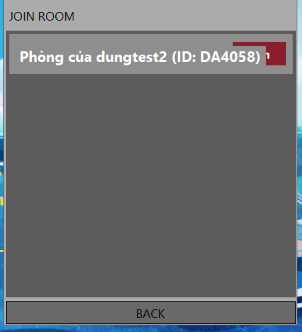
\includegraphics[height=0.22\textheight]{images/11-room-list.png}}{}
  \end{haicot}
\end{frame}

% ============================================================
% SLIDE 13. Trận đấu
% ============================================================
\begin{frame}[t,label=game]{Một trận đấu: luồng gói tin và luật chơi}
  \begin{haicot}{0.52}
    \centering
    \resizebox{\linewidth}{!}{%
    \begin{tikzpicture}[
      life/.style={dashed, color=skyblue, thick},
      msg/.style={-{Stealth[length=1.8mm]}, thick, color=brandblue},
      lab/.style={font=\tiny, fill=bgblue, inner sep=1pt}]
      \node[draw=inkblue, fill=paleblue, rounded corners=2pt, thick, minimum width=1.6cm, font=\scriptsize\bfseries] (a) at (0,0) {Chủ phòng};
      \node[draw=inkblue, fill=gold!45, rounded corners=2pt, thick, minimum width=2.0cm, font=\scriptsize\bfseries] (s) at (4.2,0) {Server};
      \node[draw=inkblue, fill=paleblue, rounded corners=2pt, thick, minimum width=1.6cm, font=\scriptsize\bfseries] (b) at (8.4,0) {Khách};
      \draw[life] (a.south) -- (0,-5.5); \draw[life] (s.south) -- (4.2,-5.5); \draw[life] (b.south) -- (8.4,-5.5);
      \draw[msg] (0,-0.75) -- node[lab, above]{\texttt{PlaceShipsRequest} + \texttt{PlayerReady}} (4.2,-0.75);
      \draw[msg] (8.4,-1.25) -- node[lab, above]{\texttt{PlaceShipsRequest} + \texttt{PlayerReady}} (4.2,-1.25);
      \draw[msg] (4.2,-1.95) -- node[lab, above]{\texttt{GameStart} + \texttt{TurnChange}} (0,-1.95);
      \draw[msg] (4.2,-1.95) -- node[lab, above]{\texttt{GameStart} + \texttt{TurnChange}} (8.4,-1.95);
      \draw[msg] (0,-2.7) -- node[lab, above]{\texttt{FireShotRequest(X,Y)}} (4.2,-2.7);
      \draw[msg] (4.2,-3.35) -- node[lab, above]{\texttt{ShotResult} (trúng, hụt, chìm)} (0,-3.35);
      \draw[msg] (4.2,-3.35) -- node[lab, above]{\texttt{ShotResult}} (8.4,-3.35);
      \draw[msg] (4.2,-4.1) -- node[lab, above]{hụt hoặc quá 30s: \texttt{TurnChange}} (0,-4.1);
      \draw[msg] (4.2,-4.1) -- node[lab, above]{\texttt{TurnChange}} (8.4,-4.1);
      \draw[msg] (4.2,-4.95) -- node[lab, above]{hết tàu: \texttt{GameOver}} (0,-4.95);
      \draw[msg] (4.2,-4.95) -- node[lab, above]{\texttt{GameOver}} (8.4,-4.95);
    \end{tikzpicture}%
    }
  \sang{0.46}
    \begin{khung}{LUẬT CHƠI}
      \textbf{Bắn từng phát.} Trúng thì bắn tiếp, hụt thì đổi lượt; quá \textbf{30 giây} không bắn cũng đổi lượt. Chìm hết 5 tàu (17 ô) thì thắng.
    \end{khung}
    \begin{khung}{SERVER QUYẾT ĐỊNH, CHỐNG GIAN LẬN}
      \begin{itemize}\setlength{\itemsep}{1pt}
        \item Xếp tàu phải đúng \textbf{5 tàu cỡ 5, 4, 3, 3, 2}, không ra ngoài lưới, không chồng nhau.
        \item Bắn ngoài lượt bị bỏ qua; bắn ra ngoài hoặc trùng ô trả \texttt{IsValid = false}, giữ lượt.
        \item Server tự phán trúng, hụt, chìm và ghi lại từng phát bắn.
      \end{itemize}
    \end{khung}
    \begin{khung}{MẤT KẾT NỐI GIỮA TRẬN}
      Heartbeat: Server gửi \texttt{Ping} mỗi \textbf{5 giây}; quá \textbf{15 giây} không có \texttt{Pong} thì ngắt phiên. Người ở lại nhận \texttt{GameOver} (thắng).
    \end{khung}
  \end{haicot}
\end{frame}

% ============================================================
% SLIDE 14. Database: lược đồ
% ============================================================
\begin{frame}[t,label=db_erd]{Cơ sở dữ liệu: lược đồ quan hệ}
  \centering
  \resizebox{0.96\textwidth}{!}{%
  \begin{tikzpicture}[
    ent/.style={draw=inkblue, fill=white, rounded corners=2pt, thick, align=left,
                font=\scriptsize, inner sep=3.5pt},
    arr/.style={thick, color=brandblue},
    lab/.style={font=\tiny, fill=bgblue, inner sep=1pt}]
    \node[ent] (u) at (0,0)    {\textbf{Users} (PK: \texttt{Id})\\[1pt]
      \underline{\texttt{Id}} : TEXT (GUID)\\
      \texttt{Username} : TEXT (\textbf{UNIQUE})\\
      \texttt{Password} : TEXT (BCrypt)\\
      \texttt{Email} : TEXT NULL\\
      \texttt{Wins, Losses, Score} : INT\\
      \texttt{Condition} : INT/BOOL\\
      \texttt{UserId} : TEXT NULL (FK $\rightarrow$ \texttt{Users.Id})};
    \node[ent] (m) at (6.0,0)  {\textbf{Matches} (PK: \texttt{Id})\\[1pt]
      \underline{\texttt{Id}} : INT (AUTO)\\
      \texttt{Player1Id} : TEXT (FK, RESTRICT)\\
      \texttt{Player2Id} : TEXT NULL (FK, RESTRICT)\\
      \texttt{WinnerId} : TEXT NULL (FK, RESTRICT)\\
      \texttt{StartTime} : TEXT/TIMESTAMP\\
      \texttt{EndTime} : TEXT/TIMESTAMP NULL};
    \node[ent] (d) at (12.2,0) {\textbf{MatchDetails} (PK: \texttt{Id})\\[1pt]
      \underline{\texttt{Id}} : INT (AUTO)\\
      \texttt{MatchId} : INT (FK, CASCADE)\\
      \texttt{PlayerId} : TEXT (FK, RESTRICT)\\
      \texttt{X\_Coordinate, Y\_Coordinate} : INT\\
      \texttt{IsHit} : INT/BOOL\\
      \texttt{TurnTime} : TEXT/TIMESTAMP};
    \draw[arr] (u.east) -- node[lab, above]{1--N (P1/P2/Winner)} (m.west);
    \draw[arr] (m.east) -- node[lab, above]{1--N (\texttt{MatchId})} (d.west);
    \draw[arr] (u.south) to[out=-12,in=-168] node[lab, below]{1--N (\texttt{MatchDetails.PlayerId})} (d.south);
    \draw[arr] (u.north west) to[out=55,in=125,looseness=0.7] node[lab, above]{\texttt{UserId} (tự tham chiếu)} (u.north east);
  \end{tikzpicture}%
  }
  \vspace{0.05cm}
  \begin{haicot}{0.49}
    \begin{khung}[equal height group=dbe]{HAI CHẾ ĐỘ (\texttt{AppDbContext.cs}, \texttt{BATTLESHIP\_DB})}
      \begin{itemize}\setlength{\itemsep}{0.5pt}
        \item \textbf{SQLite} (offline): \texttt{EnsureCreated()} tạo \texttt{battleship.db}; kiểm tra \texttt{pragma\_table\_info} để tự thêm cột \texttt{Email}.
        \item \textbf{PostgreSQL (Supabase)}: kiểm tra \texttt{information\_schema.tables} rồi gọi \texttt{CreateTables()}; thêm \texttt{Email} bằng \texttt{IF NOT EXISTS}; bật \texttt{LegacyTimestampBehavior}.
      \end{itemize}
    \end{khung}
  \sang{0.49}
    \begin{luuy}[equal height group=dbe]{VIEW BẢNG XẾP HẠNG, RLS \& TRẠNG THÁI GHI}
      \begin{itemize}\setlength{\itemsep}{0.5pt}
        \item \texttt{supabase\_setup.sql} bật \textbf{RLS} và \texttt{REVOKE ALL} trên 3 bảng gốc; chỉ mở \texttt{SELECT} cho view \texttt{public.leaderboard} (\texttt{Username, Wins, Losses, Score}).
        \item \textbf{Thực tế 27/11}: chỉ bảng \texttt{Users} đang đọc/ghi. Bảng \texttt{Matches} và \texttt{MatchDetails} \textbf{chưa có code ghi dữ liệu}.
      \end{itemize}
    \end{luuy}
  \end{haicot}
\end{frame}

% ============================================================
% SLIDE 15. Database: các bảng
% ============================================================
\begin{frame}[t,label=db_tables]{Cơ sở dữ liệu: các bảng và nơi đọc, ghi}
  \begin{khung}{CẤU TRÚC 3 BẢNG THẬT (TỪ \texttt{sqlite\_master} ĐỐI CHIẾU \texttt{supabase\_setup.sql})}
    \tiny
    \renewcommand{\arraystretch}{1.05}
    \begin{tabularx}{\linewidth}{@{}l >{\raggedright\arraybackslash}p{6.0cm} Y@{}}
      \toprule \textbf{Bảng} & \textbf{Cột \& Kiểu (SQLite / PostgreSQL)} & \textbf{Ý nghĩa \& Ràng buộc} \\ \midrule
      \texttt{Users} &
        \texttt{Id} (TEXT PK), \texttt{Username} (TEXT UNIQUE), \texttt{Password} (TEXT), \texttt{Email} (TEXT NULL), \texttt{Wins/Losses/Score} (INT), \texttt{Condition} (INT/BOOL), \texttt{UserId} (TEXT NULL FK) &
        Tài khoản, hash BCrypt, email OTP, điểm số. \texttt{UserId} (FK tự tham chiếu \texttt{Users.Id}) do EF Core sinh từ \texttt{ICollection<User> Friend} (không tạo bảng trung gian). \\
      \texttt{Matches} &
        \texttt{Id} (INT AUTO PK), \texttt{Player1Id} (TEXT FK), \texttt{Player2Id} (TEXT NULL FK), \texttt{WinnerId} (TEXT NULL FK), \texttt{StartTime} (TEXT/TS), \texttt{EndTime} (TEXT/TS NULL) &
        Thông tin trận đấu (3 khóa ngoại trỏ \texttt{Users.Id}, \texttt{ON DELETE RESTRICT}). \textbf{Chưa ghi dữ liệu.} \\
      \texttt{MatchDetails} &
        \texttt{Id} (INT AUTO PK), \texttt{MatchId} (INT FK CASCADE), \texttt{PlayerId} (TEXT FK RESTRICT), \texttt{X\_Coordinate/Y\_Coordinate} (INT), \texttt{IsHit} (INT/BOOL), \texttt{TurnTime} (TEXT/TS) &
        Lịch sử từng phát bắn của trận đấu (khớp \texttt{ShotRecord} trên Server). \textbf{Chưa ghi dữ liệu.} \\
      \bottomrule
    \end{tabularx}
  \end{khung}
  \begin{khung}{CHỨC NĂNG ĐỌC / GHI DỮ LIỆU TRONG CODE}
    \tiny
    \renewcommand{\arraystretch}{1.05}
    \begin{tabularx}{\linewidth}{@{}l l l Y@{}}
      \toprule \textbf{Chức năng} & \textbf{Bảng / View} & \textbf{Thao tác} & \textbf{Hàm xử lý} \\ \midrule
      Đăng ký & \texttt{Users} & Đọc + Ghi & \texttt{AuthHandler.HandleRegisterAsync} (kiểm tra trùng tên, thêm bản ghi mới) \\
      Đăng nhập & \texttt{Users} & Đọc & \texttt{AuthHandler.HandleLoginAsync} (lấy hash BCrypt và \texttt{Wins/Losses/Score}) \\
      Quên mật khẩu & \texttt{Users} & Đọc + Sửa & \texttt{PasswordResetHandler.HandleForgotAsync}, \texttt{HandleResetAsync} (đổi \texttt{Password}) \\
      Bảng xếp hạng & \texttt{public.leaderboard} & Chỉ đọc & \texttt{LeaderboardService.GetTopAsync} (HTTPS REST trên Supabase) \\
      Lưu lịch sử trận & \texttt{Matches}, \texttt{MatchDetails} & \textbf{Chưa ghi} & \texttt{TcpServer.cs} còn \texttt{TODO} nối sự kiện \texttt{RoomManager.OnMatchFinished} \\
      \bottomrule
    \end{tabularx}
  \end{khung}
\end{frame}

% ============================================================
% SLIDE 16. Bảo mật
% ============================================================
\begin{frame}[t,label=bm]{Thiết kế bảo mật nhiều lớp}
  \footnotesize
  \begin{tabularx}{\textwidth}{@{}l Y Y@{}}
    \toprule \textbf{Lớp} & \textbf{Biện pháp (đã chạy trên \texttt{origin/main})} & \textbf{Chống lại} \\ \midrule
    Đường truyền & AES-128-CBC, IV ngẫu nhiên 16 byte mỗi gói (\texttt{CryptoHelper}) & Nghe lén, đọc trộm gói tin \\
    Mật khẩu & BCrypt (salt, cost 11), luôn chạy với \texttt{DummyHash} nếu sai tên & Lộ mật khẩu khi rò DB, dò tên qua thời gian \\
    Đăng nhập & Khóa 60 giây sau 5 lần sai trong 5 phút (theo IP và theo tên) & Dò mật khẩu hàng loạt \\
    Đăng ký & Tối đa 5 lần / 10 phút / IP, khóa 5 phút (\texttt{\_registerLimiter}) & Tạo tài khoản rác \\
    Quên mật khẩu & Mã 6 số ngẫu nhiên (10 phút), chờ 60s, \texttt{FixedTimeEquals}, sai 5 lần hủy & Dò mã OTP, gửi thư rác \\
    Phiên & \texttt{PacketRouter} chặn gói ngoài \texttt{PublicTypes}; 1 phiên/tài khoản & Gửi lệnh khi chưa xác thực, đăng nhập trùng \\
    Dữ liệu & RLS + \texttt{REVOKE ALL} trên 3 bảng; chỉ mở \texttt{SELECT} view \texttt{leaderboard} & Đọc trực tiếp bảng \texttt{Users} qua REST \\
    Luật chơi & Server kiểm tra 5 tàu, đúng lượt, phán Hit/Miss/Sunk/GameOver & Client gian lận \\
    \bottomrule
  \end{tabularx}
\end{frame}

% ============================================================
% SLIDE 17. Tính năng đặc biệt
% ============================================================
\begin{frame}[t,label=dacbiet]{Tính năng đặc biệt: tối ưu khi đông người chơi}
  \begin{haicot}{0.49}
    \begin{khung}[equal height group=db]{VẤN ĐỀ KHI CÓ NHIỀU NGƯỜI CHƠI}
      \begin{itemize}\setlength{\itemsep}{1.5pt}
        \item Phát gói (\texttt{BroadcastAsync}) gửi tới từng phiên; nếu không có hàng đợi giới hạn, client chậm gây ùn ứ hoặc tốn RAM.
        \item Hiện mỗi gói vẫn \textbf{mã hóa AES lại} cho từng người nhận trong \texttt{ProcessSendQueueAsync}.
        \item Nhiều người đăng nhập cùng lúc cùng chạy BCrypt (cố tình chậm) làm tăng tải CPU.
        \item Một tiến trình Server duy nhất có giới hạn về CPU và số kết nối.
      \end{itemize}
    \end{khung}
  \sang{0.49}
    \begin{khung}[equal height group=db]{HƯỚNG TỐI ƯU: ĐO TRƯỚC, SỬA, ĐO SAU}
      \begin{itemize}\setlength{\itemsep}{1.5pt}
        \item \textbf{Đã xong}: mỗi \texttt{ClientSession} có \texttt{BoundedChannel} giới hạn \textbf{1000 gói} và 1 Task ghi nền; đầy hàng thì ngắt riêng client chậm (PR \#59).
        \item \textbf{Đang làm}: mã hóa một lần cho mỗi lần phát, giới hạn số BCrypt chạy đồng thời, gộp thông báo Online.
        \item \textbf{Kiểm thử}: viết bộ mô phỏng 50--200 client đo độ trễ, RAM, CPU trước và sau khi tối ưu.
      \end{itemize}
    \end{khung}
  \end{haicot}
  \begin{ketluan}
    Kế hoạch mở rộng (nếu kịp trước hạn): bộ điều phối Round-Robin cho nhiều Server và kết nối lại giữa trận bằng token (giữ ván 15s).
  \end{ketluan}
\end{frame}

% ============================================================
% SLIDE 18. Độ phức tạp
% ============================================================
\begin{frame}[t,label=phuctap]{Phân tích độ phức tạp các chức năng}
  \begin{haicot}{0.49}
    \begin{khung}[equal height group=pt]{PHỨC TẠP THẤP VÀ VỪA}
      \textbf{Thấp (theo mẫu sẵn):}
      \begin{itemize}\setlength{\itemsep}{1pt}
        \item Đăng ký, đăng nhập, Profile: nhận gói, kiểm tra, đọc/ghi bảng \texttt{Users}.
        \item Chat, bảng xếp hạng: phát lại gói hoặc chỉ đọc REST.
      \end{itemize}
      \textbf{Vừa (nhiều luồng dùng chung dữ liệu):}
      \begin{itemize}\setlength{\itemsep}{1pt}
        \item Ghép trận: \texttt{ConcurrentQueue} + vé \texttt{Ticket} tránh tự ghép khi hủy rồi bấm lại.
        \item Phòng đấu: khóa \texttt{RoomLock} khi vào, rời, Kick đồng thời.
        \item Chống dò mật khẩu, 1 phiên/tài khoản: nhiều luồng cùng cập nhật bảng theo dõi.
      \end{itemize}
    \end{khung}
  \sang{0.49}
    \begin{luuy}[equal height group=pt]{PHỨC TẠP CAO (TRỌNG TÂM ĐỒ ÁN)}
      \begin{itemize}\setlength{\itemsep}{1.5pt}
        \item \textbf{Giao thức gói tin}: TCP không giữ ranh giới gói, phải tự đóng khung 4 byte, Handshake, mã hóa AES từng gói.
        \item \textbf{Luật trận trên Server}: kiểm tra 5 tàu, đúng lượt, phán trúng/hụt/chìm, quản lý Timer 30 giây bằng phiên bản \texttt{\_turnVersion}.
        \item \textbf{Mất kết nối giữa trận}: Heartbeat 5s/15s, dọn phiên an toàn, kết thúc ván không deadlock.
        \item \textbf{Chịu tải nhiều người chơi}: bảo vệ RAM bằng \texttt{BoundedChannel}, tối ưu phát gói và BCrypt.
      \end{itemize}
    \end{luuy}
  \end{haicot}
  \vspace{0.05cm}\scriptsize Đánh giá dựa trên mức độ khó khi thiết kế và lập trình; số đo tải thực tế sẽ có ở giai đoạn kiểm thử (03/12 -- 08/12).
\end{frame}

% ============================================================
% SLIDE 19. Cải tiến cuối kỳ
% ============================================================
\begin{frame}[t,label=caitien]{Cải tiến cuối kỳ so với giữa kỳ}
  \footnotesize
  \begin{tabularx}{\textwidth}{@{}l Y Y@{}}
    \toprule
    \textbf{Khía cạnh} & \textbf{Giữa kỳ (hiện tại 27/11 trên \texttt{origin/main})} & \textbf{Cuối kỳ (kế hoạch, hạn code 02/12)} \\
    \midrule
    \textbf{Hiệu năng} &
      Đã có \texttt{BoundedChannel} 1000 gói cho từng phiên (PR \#59). Mỗi người nhận vẫn mã hóa AES riêng, chưa đo tải. &
      Mã hóa 1 lần khi broadcast, giới hạn số BCrypt đồng thời, gộp thông báo Online; \textbf{đo trước/sau} với 50--200 client giả lập. \\
    \textbf{Trận đấu} &
      Đã chạy trọn vòng trận: xếp 5 tàu, Ready, bắn 1 phát/lượt, Hit/Miss/Sunk, Timer 30 giây, \texttt{GameOver}. &
      Hoàn thiện hiển thị màn sương và trải nghiệm bàn cờ; tách chat trong trận theo \texttt{RoomId}. \\
    \textbf{Đứt mạng} &
      Heartbeat Ping 5s / timeout 15s; mất kết nối giữa trận xử thắng ngay (\texttt{OpponentDisconnected}). &
      Kiểm thử rút dây mạng/End Task thực tế; kế hoạch mở rộng kết nối lại bằng token (giữ ván 15s). \\
    \textbf{Dữ liệu \& Tài khoản} &
      Đăng ký/đăng nhập, quên mật khẩu OTP (chưa thử Gmail thật), Logout phía Server; bảng \texttt{Matches/MatchDetails} chưa ghi. &
      Nối \texttt{OnMatchFinished} ghi \texttt{Matches/MatchDetails} và cập nhật \texttt{Wins/Losses/Score}; thêm nút Đăng xuất UI; thử SMTP thật. \\
    \textbf{Môi trường demo} &
      Chạy 2 Client trên cùng máy (\texttt{127.0.0.1:8000}). &
      Thêm ô nhập IP/Port trên Client + Ngrok TCP để chơi giữa hai mạng khác nhau; đóng gói self-contained. \\
    \bottomrule
  \end{tabularx}
\end{frame}

% ============================================================
% SLIDE 20. Demo
% ============================================================
\begin{frame}[label=demo]{Kịch Bản Demo}
  \begin{columns}[T]
    \begin{column}{0.62\textwidth}
      \footnotesize
      \begin{tabularx}{\textwidth}{@{}c Y c@{}}
        \toprule \textbf{\#} & \textbf{Việc làm và kết quả mong đợi} & \textbf{Hiện tại} \\ \midrule
        1 & Chạy Server: in ``Đang dùng: Supabase'' và ``Đang lắng nghe tại cổng 8000'' & \textcolor{green!50!black}{Chạy} \\
        2 & Đăng ký hai tài khoản; trên Supabase mật khẩu là chuỗi BCrypt & \textcolor{green!50!black}{Chạy} \\
        3 & Đăng nhập; sai 5 lần thì khóa 60 giây có đếm ngược & \textcolor{green!50!black}{Chạy} \\
        4 & Hai Client vào Lobby, chat sảnh, thấy nhau Online & \textcolor{green!50!black}{Chạy} \\
        5 & Cả hai bấm ``Find Opponent'': Server ghép cặp, hai bên vào phòng chờ & \textcolor{green!50!black}{Chạy} \\
        6 & Mở bảng xếp hạng (REST Supabase) & \textcolor{green!50!black}{Chạy} \\
        7 & Chơi một trận: xếp 5 tàu, bắn 1 phát/lượt, đếm 30 giây, thắng/thua & \textcolor{orange!80!black}{Cần thử} \\
        \bottomrule
      \end{tabularx}
      \vspace{0.1cm}

      \scriptsize Chạy trên cùng một máy (hai cửa sổ Client). Bảng lịch sử trận (\texttt{Matches/MatchDetails}) chưa nối ghi DB. Có phương án dự phòng chạy bằng SQLite khi mất mạng.
    \end{column}
    \begin{column}{0.34\textwidth}
      \centering
      % [ẢNH] cửa sổ Server khi khởi động
      \slideimg[\textwidth]{10-server-log.png}{Cửa sổ Server: dòng ``Đang dùng: Supabase'' và ``Đang lắng nghe tại cổng 8000''}
    \end{column}
  \end{columns}
\end{frame}

% ============================================================
% SLIDE 21. Cảm ơn
% ============================================================
{\setbeamertemplate{footline}{}
\begin{frame}[plain,label=thanks]
  \centering
  \vspace{1.2cm}
  {\bungee\color{inkblue}\fontsize{17}{21}\selectfont CẢM ƠN CÔ VÀ CÁC BẠN\\ĐÃ LẮNG NGHE}\par
  \vspace{0.5cm}
  {\bevnsemi\color{brandblue}\small Hỏi đáp (Q\&A)}\par
  \vspace{0.3cm}
  {\bevnsemi\color{footernavy}\footnotesize Hoàng $\cdot$ Đức $\cdot$ Dũng}
\end{frame}}

\end{document}
